\subsubsection{generation.domegeneration}
    Domegeneration ist dafür verantwortlich eine Kuppel (\textit{AbstractDome}) zu Generieren,
    dies geschieht mit Hilfe der Implementrierungen einer Rauschfunktion (\textit{AbstractNoiseGenerator})
    und einer Objekt Generierungsfunktion (\textit{AbstractDomeAssetGenerator}). \par
   
    \begin{figure}[htbp]
        \centering
        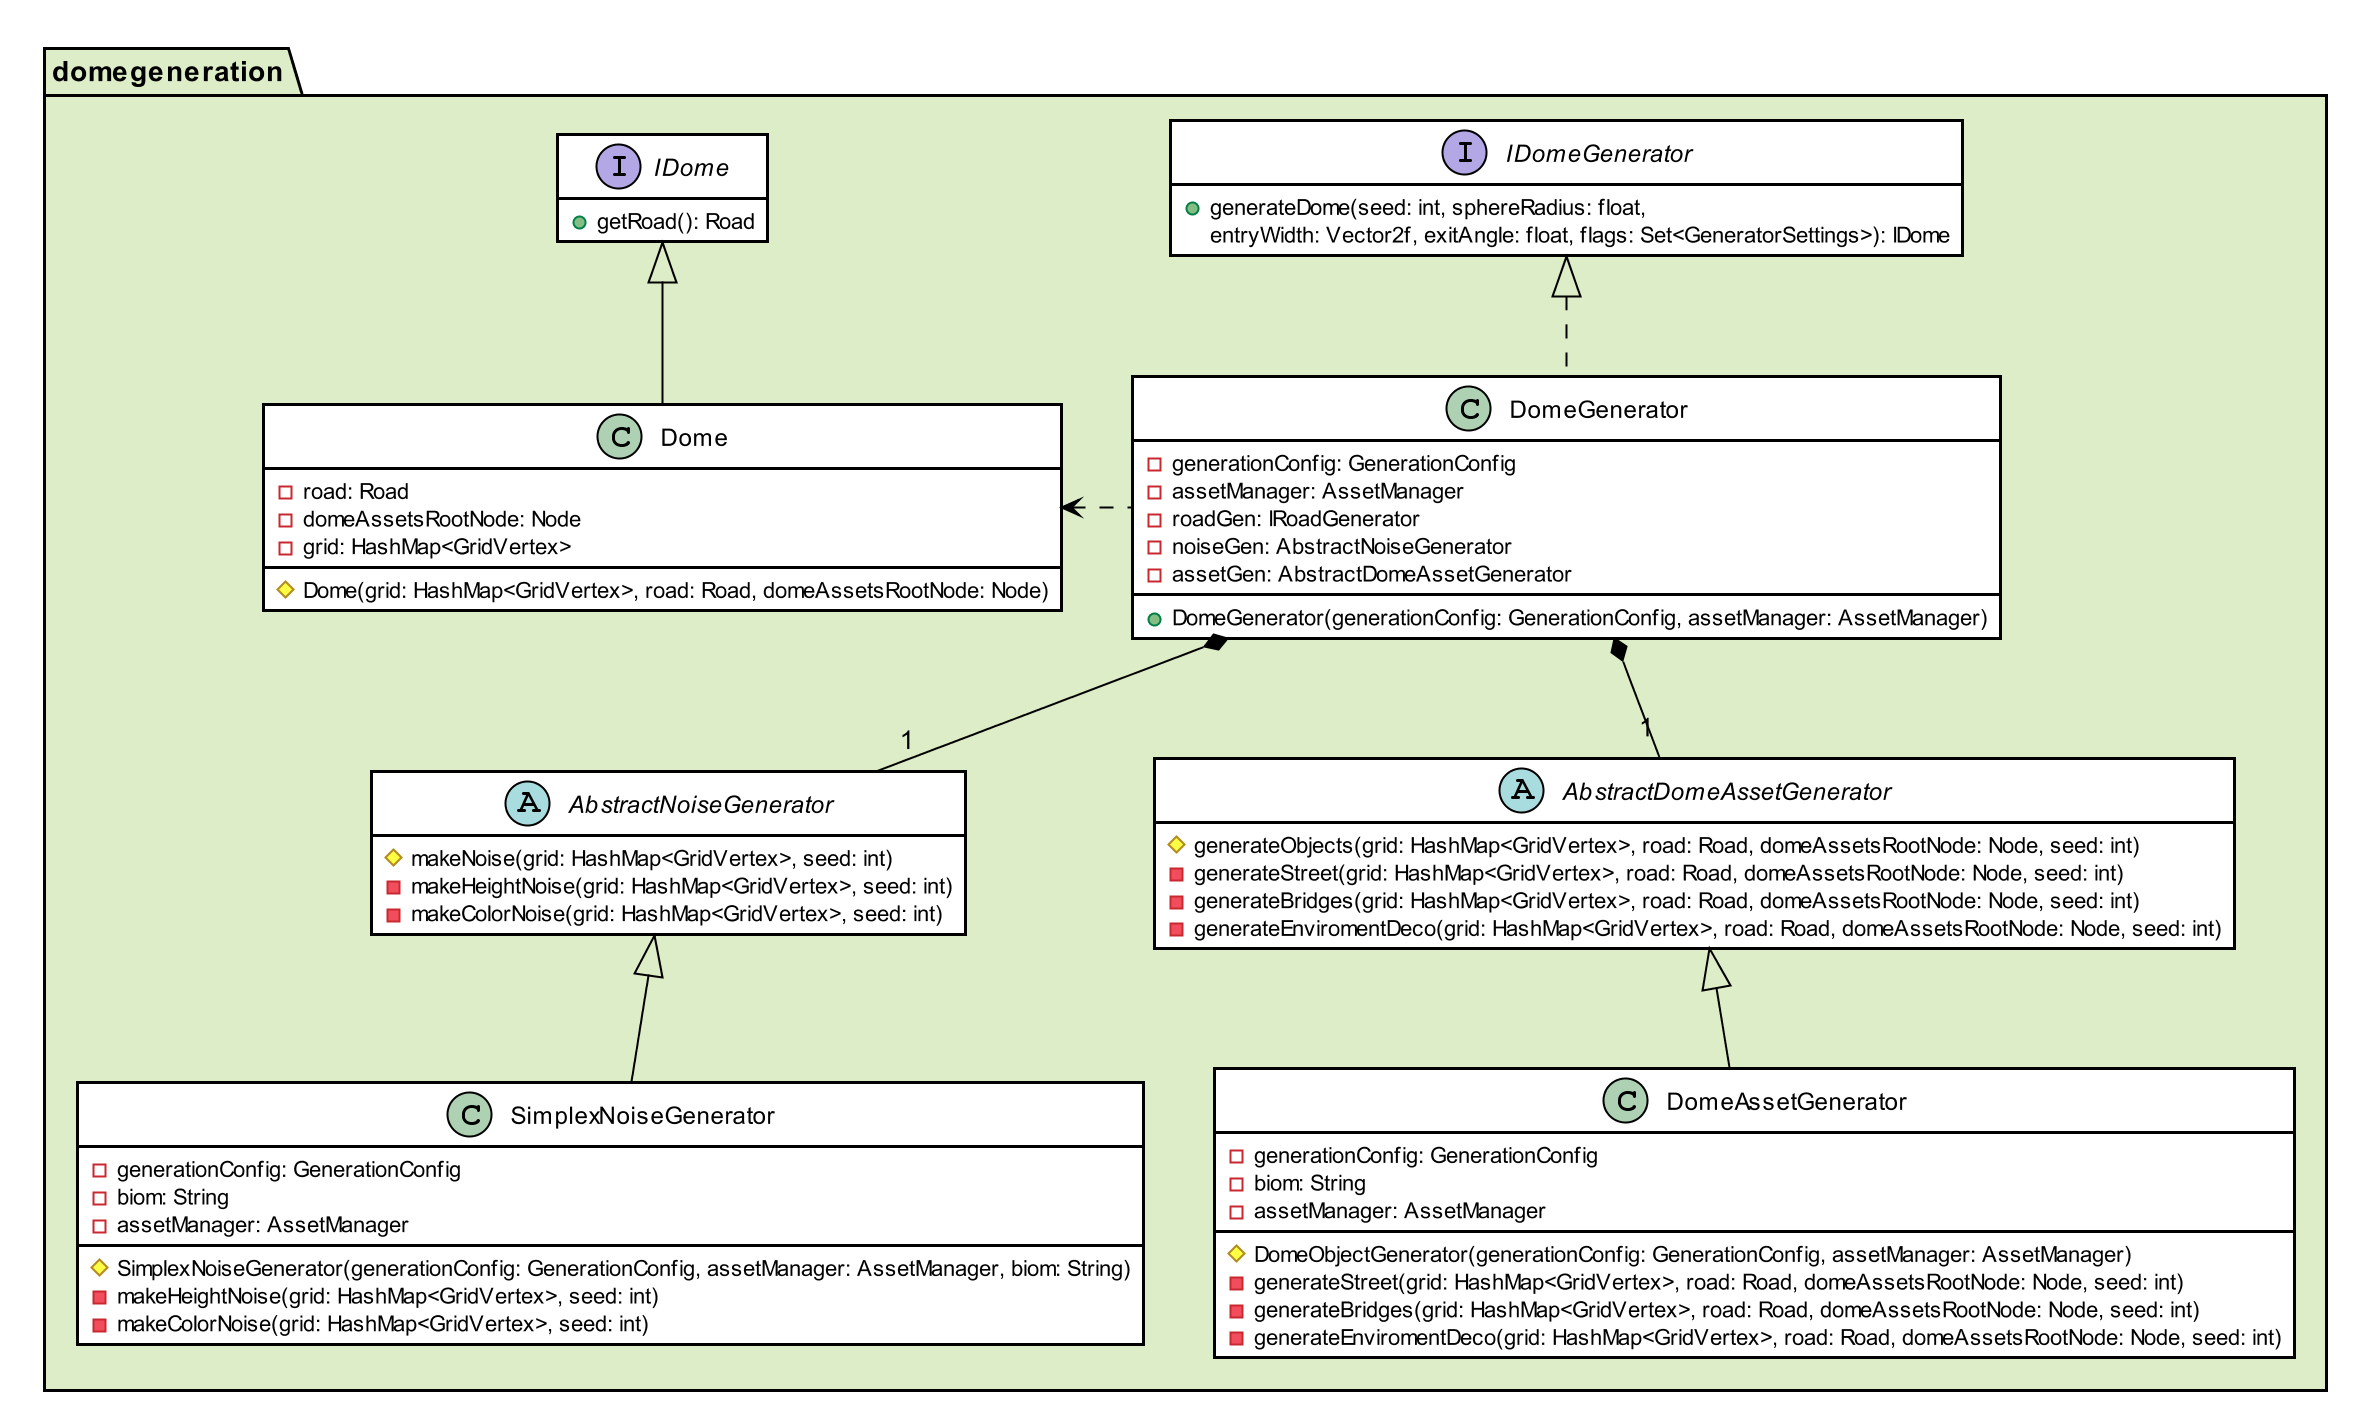
\includegraphics[width=\linewidth]{./Generierung/Bilder/domegeneration.png}
        \caption{Klassendiagramm domegeneration}
    \end{figure}


        \paragraph{\underline{IDomeGenerator}} \mbox{}\par
            Schnittstelle nach außsen, zur Genereirung einer Kupppel über welche sich der Genereirungsprozess
            anregen lässt. \textit{IDomeGenerator} bildet die abstrakte Fabrik im Entwurfmuster 'Fabrik'. \par
            
            \textbf{Methoden}					
            \begin{itemize}
                \item  \textit{+ generateDome(int seed, float sphereRadius,Vector2f entryWidth,
                                 float exitAngle, Set<GeneratorSettings> flags): IDome}
                    \begin{leftbar}[0.9\linewidth]
                        Stößt den Genereirungsprozess zu einem \textit{AbstractDome} an.\\
                        \textbf{@param seed} Zum generieren von Pseudozufallswerte.\\
                        \textbf{@param sphereRadius} Legt maximale Größe der Kuppel fest.\\
                        \textbf{@param entryWidth} Legt Dimensionen des Eingangs in die Kuppel fest.\\
                        \textbf{@param exitAngle} Legt Winkel zwischen Ein-/ und Ausgang fest, welcher angenähert
                            werden soll.\\
                        \textbf{@param flags} Menge an Präferenzen, die zur Generierung übergegben werden.\\
                        \textbf{@return} Datenstruktur, die eine Kuppel repräsentiert.
                    \end{leftbar}
            \end{itemize}


        \paragraph{\underline{DomeGenerator}} \mbox{}\par
            Konkrete Implementierung der Schnittstelle \textit{IDomeGenerator} und stellt somit die
            konkrete Fabrik im Entwurfsmuster 'Fabrik' dar welche einen konkreten \textit{Dome} generiert. \par
            
            \textbf{Attribute}
            \begin{itemize}
                \item  \textit{- GenerationConfig generationConfig} 
                    \begin{leftbar}[0.9\linewidth]
                        Datenstruktur, die Parameter für die Generierung hält.
                    \end{leftbar}
                
                \item  \textit{- AssetManager assetManager} 
                    \begin{leftbar}[0.9\linewidth]
                        Von \textit{JMonkey} vordefinierte Klasse, zum verwalten von Assets.
                    \end{leftbar}
            
                \item  \textit{- IRoadGenerator roadGen} 
                    \begin{leftbar}[0.9\linewidth]
                        Ist für die Generierung eines Streckenverlaufs verantwortlich.
                    \end{leftbar}
                
                \item  \textit{- AbstractNoiseGenerator noiseGen} 
                    \begin{leftbar}[0.9\linewidth]
                        Ist für die Generierung einer Rauschfunktion, um eine Landschaft zu erzeugen, zuständig.
                    \end{leftbar}
                
                \item  \textit{- AbstractDomeAssetGenerator assetGen} 
                    \begin{leftbar}[0.9\linewidth]
                        Verteilt verschiedenen Assets in der Landschaft, beispielsweise Dekoration.
                    \end{leftbar}
            \end{itemize}

            \textbf{Methoden}					
            \begin{itemize}
                \item  \textit{+ DomeGenerator(GenerationConfig generationConfig, AssetManager assetManager)}
                    \begin{leftbar}[0.9\linewidth]
                        Konsrtuktor von \textit{DomeGenerator}.\\
                        \textbf{@param generationConfig} Datenstruktur, die Parameter für die Generierung hält.\\
                        \textbf{@param assetManager} Von \textit{JMonkey} vordefinierte Klasse, zum verwalten von Assets.
                    \end{leftbar}
            \end{itemize}
            
            
            
            \paragraph{\underline{AbstractNoiseGenerator}} \mbox{}\par
            Definiert und implementiert die Grundvorraussetzungen für eine Rauschfuntion, 
            die eine an die Strecke angepasste Landschaft erzeugt.\par
            
            \textbf{Methoden}					
            \begin{itemize}
                \item  \textit{\# makeNoise(HashMap<GridVertex> grid, int seed)}
                    \begin{leftbar}[0.9\linewidth]
                        Generiert eine Rauschfunktion an Hand aller gegebenen Parameter, wie dem Biom, um eine Landschaft zu generieren,
                        die diesen entspricht.\\
                        \textbf{@param grid} Das Gitter der Kuppel, sodass ein Status eines \textit{GridVertex} abgerufen weren kann,
                            um die Rauschfunktion an Gegebenheiten wie Streckenhöhe anzupassen.\\
                        \textbf{@param seed} Zum generieren von Pseudozufallswerte.
                    \end{leftbar}  
            \end{itemize}



            

            \paragraph{\underline{SimplexNoisGenerator}} \mbox{}\par
            Erweitert \textit{AbstractNoiseGenerator} indem eine konkrete Rauschfunktion (\textit{SimplexNois}) implementiert wird.\par
            
            \textbf{Attribute}
            \begin{itemize}
                \item  \textit{- GenerationConfig generationConfig} 
                    \begin{leftbar}[0.9\linewidth]
                        Datenstruktur, die Parameter für die Generierung hält.
                    \end{leftbar}

                \item  \textit{- AssetManager assetManager} 
                    \begin{leftbar}[0.9\linewidth]
                        Von \textit{JMonkey} vordefinierte Klasse, zum verwalten von Assets.
                    \end{leftbar}
                
                \item  \textit{- String biom} 
                    \begin{leftbar}[0.9\linewidth]
                        Gibt an, wo im JSON - Dokument die Inforamtionen über das aktuelle Biom zu finden sind.
                    \end{leftbar}
            \end{itemize}


            \textbf{Methoden}					
            \begin{itemize}
                \item  \textit{\# SimplexNoisGenerator(GenerationConfig generationConfig,AssetManager assetManager, String biom)}
                    \begin{leftbar}[0.9\linewidth]
                        Konsrtuktor von \textit{SimplexNoisGenerator}.\\
                        \textbf{@param generationConfig} Datenstruktur, die Parameter für die Generierung hält.\\
                        \textbf{@param assetManager} Von \textit{JMonkey} vordefinierte Klasse, zum verwalten von Assets.\\
                        \textbf{@param biom} Gibt an, wo im JSON - Dokument die Inforamtionen über das aktuelle Biom stehen.
                    \end{leftbar}   
            \end{itemize}
            
            
            
            \paragraph{\underline{AbstractDomeAssetGenerator}} \mbox{}\par
            Definiert und implementiert die MindestAnforderungen eines AssetGenerators für eine Kuppel. Diese sind dafür zuständig Object, 
            die auf die Landschaft angepasst sind, zu erzeugen.\par

            \textbf{Methoden}					
            \begin{itemize}
                \item  \textit{\# generateObjects(HashMap<GridVertex> grid, Road road, Node domeAssetsRootNode, int seed)}
                    \begin{leftbar}[0.9\linewidth]
                        Erzeugt und verteilt Objekte an Hand der Eigenschaften der durch \textit{grid} mitgegebenen Landschaft. Dies wird schrittweise innerhalb
                            einer Schablonenmethode durchgeführt.\\
                        \textbf{@param grid} Repräsentiert eine Kuppel, indem für jedes Feld (\textit{GridVertex}) Eigenschaften gespeichert sind.\\
                        \textbf{@param road} Repräsentiert die Straße in einer Kuppel.\\
                        \textbf{@param domeAssetsRootNode} Node wie in JMonkey verwendet, hier werden alle Objekte für die Kuppel angehängt.\\
                        \textbf{@param seed} Zum generieren von Pseudozufallswerte.
                    \end{leftbar}  
            \end{itemize}
            
            
            
            \paragraph{\underline{DomeAssetGenerator}} \mbox{}\par
            Erweitert \textit{AbstractDomeAssetGenerator} in dem die Erzeugung von Objekten hier in einer konkreten Strategie Umgesetzt wird.\par
            
            \textbf{Attribute}
            \begin{itemize}
                \item  \textit{- GenerationConfig generationConfig} 
                    \begin{leftbar}[0.9\linewidth]
                        Datenstruktur, die Parameter für die Generierung hält.
                    \end{leftbar}

                    \item  \textit{- String biom} 
                    \begin{leftbar}[0.9\linewidth]
                        Gibt an, wo im JSON - Dokument die Inforamtionen über das aktuelle Biom zu finden sind.
                    \end{leftbar}
                
                \item  \textit{- AssetManager assetManager} 
                    \begin{leftbar}[0.9\linewidth]
                        Von \textit{JMonkey} vordefinierte Klasse, zum verwalten von Assets.
                    \end{leftbar}
            \end{itemize}

            \textbf{Methoden}					
            \begin{itemize}
                \item  \textit{\# DomeObjectGenerator(GenerationConfig generationConfig,String biom, AssetManager assetManager)}
                    \begin{leftbar}[0.9\linewidth]
                        Konsrtuktor für \textit{DomeObjectGenerator}.\\
                        \textbf{@param generationConfig} Datenstruktur, die Parameter für die Generierung hält.\\
                        \textbf{@param biom} Gibt an, wo im JSON - Dokument die Inforamtionen über das aktuelle Biom stehen.\\
                        \textbf{@param assetManager} Von \textit{JMonkey} vordefinierte Klasse, zum verwalten von Assets.
                    \end{leftbar}   
            \end{itemize}
            
            
            
            \paragraph{\underline{IDome}} \mbox{}\par
            Implementiert \textit{ISceneItem}. Definiert die Grundfunktionalität der Datenstruktur einer Kuppel.\par
            
            \textbf{Methoden}					
            \begin{itemize}
                \item  \textit{+ generateSceneGraph(): Node}
                    \begin{leftbar}[0.9\linewidth]
                        Berechnet Scenegraph der Kuppel und gibt ihn zurück.\\
                        \textbf{@return}  Verwendet wie in \textit{JMonkey}, wird übergeben um den Tunnel in einer Szene darzustellen.
                    \end{leftbar}

                \item  \textit{+ getRoad(): Road}
                    \begin{leftbar}[0.9\linewidth]
                        Gibt die Straße (\textit{Road}), die durch die Kuppel verläuft, zurück.\\
                        \textbf{@return} Repräsentiert die Straße in der Kuppel.
                    \end{leftbar}    
            \end{itemize}
            
            
            \pagebreak
            \paragraph{\underline{Dome}} \mbox{}\par
            Implementiert \textit{IDome} und bildet somit eine konkrete Datenstruktur, die eine Kuppel beschreibt.
            \textit{Dome} stellt das Konkrete Produkt im Entwurfmuster 'Fabrik'.\par
            
            \textbf{Attribute}
            \begin{itemize}
                \item  \textit{- HashMap<GridVertex> grid} 
                    \begin{leftbar}[0.9\linewidth]
                        Repräsentiert eine Kuppel, indem für jedes Feld (\textit{GridVertex}) Eigenschaften gespeichert sind.
                    \end{leftbar}

                \item  \textit{- Road road} 
                    \begin{leftbar}[0.9\linewidth]
                        Repräsentiert die Straße, die durch den \textit{Dome} verläuft.
                    \end{leftbar}
                
                \item  \textit{- Node domeAssetsRootNode} 
                    \begin{leftbar}[0.9\linewidth]
                        Wie in \textit{JMonkey} verwendet. Beinhaltet alle Objekten, die im \textit{Dome} verteilt sind.
                    \end{leftbar}
            \end{itemize}

            \textbf{Methoden}					
            \begin{itemize}
                \item  \textit{\# Dome(HashMap<GridVertex> gird, Road road, Node domeAssetsRootNode)}
                    \begin{leftbar}[0.9\linewidth]
                        Konsrtuktor für \textit{Dome}.\\
                        \textbf{@param grid} Ein Gitter, welches den Untergrund in der Kuppel repräsentiert. Ein \textit{GridVertex} speichert hierbei 
                            immer die Eigenschaften an einer Position.\\
                        \textbf{@param road} Repräsentiert die straße, die durch den \textit{Dome} verläuft.\\
                        \textbf{@param domeAssetsRootNode} Beinhaltet alle Objekten, die im \textit{Dome} verteilt sein werden.
                    \end{leftbar}    
            \end{itemize}